% Predlozak za pisanje diplomskog rada na PMF-MO
% Opcenita uputstva za LaTeX se mogu npr. naci na 
% http://web.math.hr/nastava/rp3, http://web.math.hr/nastava/s4-prof/latex.pdf
% NE PREPORUCA se "Ne baš tako kratak uvod u TEX", buduci se radi o vrlo starom prirucniku
% koji nije pogodan za moderne verzije LaTEXa.
% Originalna verzija "The not so short..." na http://tobi.oetiker.ch/lshort/lshort.pdf 
% je obnovljena i daje bolji uvid u moderne verzije LaTeXa

% Stil je optimiziran za kreiranje pdf dokumenta (npr. pomocu pdflatex-a, XeLaTeX-a)

\documentclass[a4paper,oneside,12pt]{memoir} % jednostrano: promijeniti twoside u oneside

% Paket inputenc omogucava direktno unosenje hrvatskih dijakritickih znakova 
% opcija utf8 za unicode (unix, linux, mac)
% opcija cp1250 za windowse
\usepackage[utf8]{inputenc}  % ukoliko se koristi XeLaTeX onda je \usepackage{xunicode}\usepackage{xltxtra}

% Stil za diplomski, unutra je ukljucena podrska za hrvatski jezik
\usepackage{diplomski}
% bibliografija na hrvatskom
\usepackage[languagenames,fixlanguage,croatian]{babelbib} % zahtijeva datoteku croatian.bdf
% hiperlinkovi 
\usepackage[pdftex]{hyperref} % ukoliko se koristi XeLaTeX onda je \usepackage[xetex]{hyperref}

\DisemulatePackage{setspace}
\usepackage{setspace}

% Odabir familije fontova:
% koristenjem XeLaTeX-a mogu se koristiti svi fontovi instalirani na racunalu, npr
% \defaultfontfeatures{Mapping=tex-text}
% \setmainfont[Ligatures={Common}]{Hoefler Text}
% ili
% \newcommand{\nas}[1]{\fontspec{Adobe Garamond Pro}\fontsize{24pt}{24pt}\color{Chocolate}\selectfont #1}
% i onda \nas{Naslov ...}
\usepackage{txfonts} % times new roman 
% Paket graphicx sluzi za manipuliranje grafikom 
\usepackage[pdftex]{graphicx} % ukoliko se koristi XeLaTeX onda je \usepackage[xetex]{graphicx}
% Paket amsmath je vec ukljucen
% Dodatno definirane matematicke okoline:
% teorem (okolina: thm), lema (okolina: lem), korolar (okolina: cor),
% propozicija (okolina: prop), definicija (okolina: defn), napomena (okolina: rem),
% slutnja (okolina: conj), primjer (okolina: exa), dokaz (okolina: proof)
% Definirane su naredbe za ispisivanje skupova N, Z, Q, R i C
% Definirane su naredbe za funkcije koje se u hrvatskoj notaciji oznacavaju drukcije 
% nego u americkoj: tg, ctg, ... (\tgh za tangens hiperbolni)
% Takodjer su definirane naredbe za Ker i Im (da bi se razlikovala od naredbe za imaginarni dio kompleksnog
% broja, naredba se zove \slika).

\pagestyle{headings}
% uz paket fancyhdr mogu se lako kreirati fancy zaglavlja i podnozja



% Podaci koje treba unijeti
\title{DNA kriptografija}
\author{Antonio Kovačić}
\advisor{prof. dr. sc. Andrej Dujella}  % obavezno s titulom (prof. dr. sc ili doc. dr. sc.)
\date{srpanj, 2014.}  % oblika mjesec, godina

% Moguce je unijeti i posvetu
% Ukoliko nema posvete, dovoljno je iskomentirati/izbrisati sljedeci redak 
\dedication{Ovaj diplomski rad posvećujem svojim roditeljima, sestri, braći, prijateljima, mentoru, profesorima, kolegama s faksa, kao i svim ljudima koji su doprinijeli kako mom intelektualnom rastu, tako i mom rastu kao cjelovite osobe.}

\begin{document}

% Naredna frontmatter generira naslovnu stranicu, stranicu za potpise povjerenstva, eventualnu posvetu i sadrzaj
% Moze se iskomentirati ukoliko nije u pitanju konacna verzija
\frontmatter

% Tekst diplomskog ...
\begin{spacing}{1.5}
% Diplomski rad treba poceti s uvodnim poglavljem  
\begin{intro}

U današnje vrijeme svjedoci smo nagloga porasta razmjene podataka. Naglim napretkom današnjih računala, javila se potreba za povećanjem sigurnosti, odnosno zaštite podataka, koji putuju preko komunikacijskog kanala. Današnji kriptosustavi omogućuju siguran prijenos takvih podataka, a ključ njihovog razbijanja zapravo leži u faktoriziranju nekog \textit{velikog} broja (na primjer \textsc{RSA} kriptosustav). Na današnjim računalima, takav problem nije lako riješiv - pa su ti sustavi još uvijek sigurni. Razvojem novih teoretskih modela računala - koji se pokušavaju i u praksi realizirati - uočeno je da problem faktorizacije neće biti više takav problem. Primjer jednog takvog računala je kvantno računalo za kojeg postoji algoritam (\textit{Shorov algoritam}) koji faktorizira broj u polinomnom vremenu.
Time se javila potreba za osmišljanjem  novih teoretskih modela računala - odnosno kriptosustava - koji bi bili otporni na kvantno izračunavanje - ne bi se mogli probiti uporabom kvantnog računala u nekom razumnom vremenu. Takve kriptosustave ćemo zvati \textit{kvantno rezistentnima}.
Tema ovog diplomskog rada biti će DNA kriptografija. Kratko rečeno, radi se o teoretskom modelu kriptografskog sustava koji pomoću DNA izračunavanja šifrira podatke. Prednost takvog sustava jest upravo što je kvantno rezistentan.\\[0.2cm]
U ovom radu najprije ćemo se ukratko upoznati s pojmom DNA računala, odnosno DNA izračunavanja, složenosti DNA računala te algoritmom za enkripciju, odnosno dekripciju podataka pomoću DNA računala.
\end{intro}
\chapter{DNA računalo}
\section{DNA izračunljivost}
DNA stroj, kao ni DNA izračunavanje nećemo striktno definirati već će definicija biti opisna - u definiciji ćemo reći koje operacije DNA stroj može izvršavati, i što pri tome mora biti zadovoljeno.\\ Prije nego definiramo DNA stroj moramo definirati neke pojmove iz logike sudova i kombinatorike.
\begin{defn}
\textbf{Alfabet} je proizvoljan konačan skup, čije elemente nazivamo \textbf{simboli}.\\
Neka je $n \in \mathbb{N}$ proizvoljan te $A$ proizvoljan alfabet, proizvoljni element $w \in A^n$ zovemo \textbf{riječ alfabeta A}. Neka su $s_1,..., s_n \in A$, riječ $w=(s_1,...,s_n)$ alfabeta A još zapisujemo kao $w=s_1s_2...s_n$. Smatramo da postoji riječ alfabeta A, koju ćemo označavati s $\varepsilon$, koja se ne sastoji ni od jednog simbola i zovemo je \textbf{prazna riječ}. Po dogovoru smatramo da je $A^0=\{\varepsilon\}$. Skup svih riječi alfabeta $A$ označavamo sa $A^*$. Neka su $a=a_1...a_m$, te, $b=b_1...b_k \in A^*$, kažemo da je riječ $c \in A^*$ nastala \textbf{konkatenacijom} riječi $a$ i $b$ ako vrijedi $c=ab=a_1...a_mb_1...b_k$. Kažemo da je riječ $c \in A^*$ podriječ riječi $a \in A^*$, ako postoje riječi $b, d \in A^*$ tako da je $a=bcd$. \textbf{Duljina riječi} se definira kao funkcija $d:A^*\to \mathbb{N}$ sa:
\begin{align*}
	d(\varepsilon) :&= 0 \\
	d(wa) :&= d(w)+1
\end{align*}
\end{defn}
\begin{defn}
Neka je S proizvoljan konačan skup, a $m:S \to \mathbb{N}$ proizvoljna funkcija. \textbf{Multiskup M na skupu S} je uređeni par $M=(S,m)$. Za proizvoljan $x\in S$, $m(x)$ zovemo \textbf{kratnost} od $x$. \textbf{Kardinalnost multiskupa M} (broj elemenata), u oznaci $|M|$, se definira kao:
\[|M|:=\sum_{x \in S} m(x)\]
\end{defn}
\begin{defn}
 \textbf{DNA lanac} je proizvoljna riječ alfabeta \{A (adenin), G (gvanin), T(timin), C (citozin)\}. DNA stroj se sastoji od konstantnog broja konačnih skupova koje nazivamo \textbf{epruvete}, a čiji su elementi DNA lanci. Za proizvoljnu epruvetu K DNA stroja definiramo multiskup $MulS(K)$ kao multiskup svih riječi koje predstavljaju DNA lance sadržane u epruveti K. U DNA stroju su definirane slijedeće instrukcije:
    \begin{itemize}
        \item Kopiraj($K_1$,$K_2$) $\to$ uz pretpostavku da je $K_2$ = $\emptyset$ , kopira MulS($K_1$) u MulS($K_2$) time više $K_2$ nije prazan
        \item Spoji($K_1$, $K_2$, $K$) $\to$ uz pretpostavku da $K$=$\emptyset$: \[MulS(K)=MulS(K_1)\bigcup MulS(K_2) \]
        \item Uoči($K$) $\to$ ispituje je li $MulS(K)\neq\emptyset$, ako je rezultat operacije je $\top$, inače $\bot$. Također se može pročitati sadržaj epruvete $MulS(K)$.
        \item Odvoji(K,w) $\to$ za skup $K$ i riječ $w$ (iz $MulS(K)$) izbacuje sve riječi iz $K$ koje kao podriječ ne sadrže riječ $w$
        \item Izvadi(K,w) $\to$ $K\backslash Odvoji(K,w)\to $izbacuje sve riječi iz $K$ koje sadrže $w$
        \item Odvoji\textunderscore Pref(K,w) $\to$ izbacuje sve riječi iz K koje ne sadrže w kao prefiks
        \item Odvoji\textunderscore Suff(K,w) $\to$ izbacuje sve riječi iz K koje ne sadrže w kao sufiks
        \item Proširi(K) $\to$ multiskupu MulS(K) još jednom dodaje elemente od K
        \item Izdvoji\textunderscore po\textunderscore duljini(K, l) $\to$ iz K izbacuje sve riječi čija je duljina različita od l
        \item Konkatenacija(K) $\to$ na slučajan način izvodi operaciju konkatenacije nad riječima iz MulS(K) tako da duljina novonastalih riječi ne bude veća od neke konstante, a vraća multiskup koji sadrži sve riječi nastale tom konkatenacijom. Vjerojatnost nastajanja duljih riječi je veća. Ukoliko MulS(K) prije izvođenja ove operacije nad epruvetom K sadrži veliki broj kopija svake od riječi, tada će MulS(K) nakon izvođenja ove operacije nad epruvetom K sadržavati sve moguće kombinacije elemenata iz K.
            \begin{itemize}
                \item \textbf{Biološki komplement} DNA lanca H definiramo kao DNA lanac koja ima jednako znakova kao i H, ali je svaki znak A zamijenjen znakom T, a svaki znak C znakom G i obratno, i označavamo je s $\overline{H}$
                \item Neka riječ H ima duljinu $n \in 2\mathbb{N}$, tada definiramo \textbf{biološki prefiks} riječi H kao biološki komplement riječi sastavljene od prvih $\frac{n}{2}$ znakova iz H, slično definiramo i \textbf{biološki sufiks} riječi H kao biološki komplement riječi sastavljene od zadnjih $\frac{n}{2}$ znakova riječi H
                \item Smatramo da je operacija konkatenacije nad riječima H i J dopuštena ako postoji riječ L takva da je biološki sufiks od H prvih $\frac{n}{2}$  znakova od L, a biološki prefiks od J prvih $\frac{n}{2}$ znakova od L
            \end{itemize}
    \item Izreži(K) $\to$ na slučajan način “skraćuje” riječi iz MulS(K) do neke fiksne duljine
    \item Izaberi(K) $\to$ na slučajan način iz MulS(K) izabire neku riječ te “generira” novi skup sastavljen od samo te riječi

    \end{itemize}
    \textbf{Program za DNA stroj} definiramo kao konačan niz gornje navedenih instrukcija. U svakom koraku programa se može izvesti točno jedna instrukcija.  Kažemo da program P za DNA stroj \textbf{izračunava} funkciju $f:S \subseteq N^k \to \N$ ako vrijedi:\\
$\vec{x}=(x_1,...,x_k) \in S$ ako i samo ako program P za DNA stroj s ulazom  $\vec{x}$ (reprezentiranim pomoću DNA lanaca) u epruveti K završi s izvršavanjem te na kraju izvršavanja vrijedi $Detect(K)=\top$ te je pri tome $K=\{f(\vec{x})\}$.\\
Kažemo da je funkcija $f:\N \to N$ \textbf{DNA izračunljiva} ako postoji program za DNA stroj koji ju izračunava.
\end{defn}
\begin{rem}
Vidimo da se sve ove operacije izvršavaju nad jednom epruvetom u jednom koraku, odnosno multiskupom $MulS(K)$. Što je veća kardinalnost multiskupa $MulS(K)$, to se više operacija na riječima izvrši istovremeno, a u stvarnom svijetu sve te operacije imaju svoje "biokemijske analogone" - biokemijske reakcije. Takvo računalo zapravo možemo interpretirati kao superračunalo s izuzetno velikim brojem procesora. U pozadini svega toga se zapravo krije masivni paralelizam. Memoriju DNA računala zapravo predstavljaju epruvete. Jasno je odakle naziv epruvete.\\
Uočimoo da je $MulS(K)$ definiran nad konačnim skupom pa je i on konačan - no vidimo da se on zapravo može proširiti nizom operacija \textit{Proširi} tako da je njegov kardinalitet izrazito velikog reda (nadeksponencijalnog) , ali u praksi se već sada zaključuje da to neće biti uvijek moguće - naime broj DNA lanaca u epruveti (laboratorijskoj) biti će ograničen volumenom te epruvete.\\
Uočimo da operacija konkatenacije uključuje vjerojatnosni efekt - \textit{vjerojatnost nastajanja duljih riječi konkatenacijom je veća} - odnosno dvije riječi iz skupa $K$ koje će se konkatenirati neće biti izabrane na slučajan način - već tako da se pokuša dobiti riječ maksimalne duljine (maksimalna duljina je određena nekom konstantom). Iz toga očito možemo vidjeti da sam ishod DNA računanja nije sasvim siguran  - no u praksi se pokazuje (pri sintezi DNA lanaca) da je to moguće - u tu svrhu je i uvedena pretpostavka da će  se, ukoliko $MulS(K)$ sadrži velik broj kopija od svake riječi iz $K$, dobiti svaka moguća konkatenacija riječi iz $K$.
\end{rem}
\section{O složenosti DNA računala}
Kako bi nešto rekli o složenosti DNA računala, najprije ćemo navesti nekoliko osnovnih definicija iz teorije složenosti algoritama, odnosno referencirati se na \cite{Sipser}.
\begin{defn}
\textbf{Turingov stroj} je uređena sedmorka $(Q, \Sigma , \Gamma , \delta, q_0, q_{DA}, q_{NE})$, gdje je redom:
\begin{itemize}
	\item Q konačan skup čije elemente nazivamo stanja
	\item $\Sigma$ je konačan skup, čije elemente nazivamo ulazni simboli, pretpostavljamo da $\Sigma$ ne sadrži "prazan simbol" kojeg označavamo sa $\varepsilon$
	\item $\Gamma$ je konačan skup kojeg nazivamo alfabet Turingovog stroja, pretpostavljamo da je $\varepsilon \in \Gamma$, te $\Sigma \subset \Gamma$
	\item $\delta : Q \times \Gamma \to Q \times \Gamma \times \{ L,D,S\}$ koju nazivamo funkcija prijelaza
	\item $q_0 \in Q$ nazivamo početnim stanjem
	\item  $q_{DA} \in Q$ nazivamo stanjem prihvaćanja
	\item $q_{NE} \in Q$ nazivamo stanjem odbijanja, te $q_{NE}\neq q_{DA}$
\end{itemize}
\end{defn}
\begin{rem} (Opis rada Turingovog stroja)\\
Turingov stroj zapravo ima četiri glavna dijela: kontrolnu jedinicu (koja zapravo oponaša dijelovanje funkcije $\delta$), beskonačnu traku, neograničenu s lijeve i desne strane, takvu da se u svakom trenutku rada stroja na jednom registru trake nalazi točno jedan simbol, memoriju u kojoj se pamti trenutačno stanje stroja te glavu za čitanje koja se u jednom koraku rada stroja može pomicati za točno jedno mjesto na traci: desno, lijevo ili ostati na istom simbolu. Glava se na početku nalazi na nekom mjestu na traci (unaprijed definiranom), zatim čita simbol. Pročitani simbol, u paru s trenutnim stanjem stroja "se šalje" u kontrolnu jedinicu. Glava nakon toga, najprije zamijeni pročitani simbol nekim drugim simbolom, stroj prelazi u novo stanje, a glava se pomiče na drugi registar (L (lijevo), D (desno)) ili ostaje na istom mjestu (S). \\
Vidimo da opisani Turingov stroj može stati u dva završna stanja $q_{DA}$, odnosno $q_{NE}$, takav Turingov stroj se naziva još odlučitelj. Uočimo da Turingov stroj ne mora nužno uvijek stati. Shematski prikaz Turingovog stroja možete vidjeti na slici \ref{fig:Turing}.\\
Nedeterministički Turingov stroj se definira na analogan način, samo što je funkcija prijelaza definirana sa: $\delta : Q \times \Gamma \to \mathcal{P}(Q \times \Gamma \times \{L,D,S\})$. 
\end{rem}
\begin{figure}[h!t]
\centering 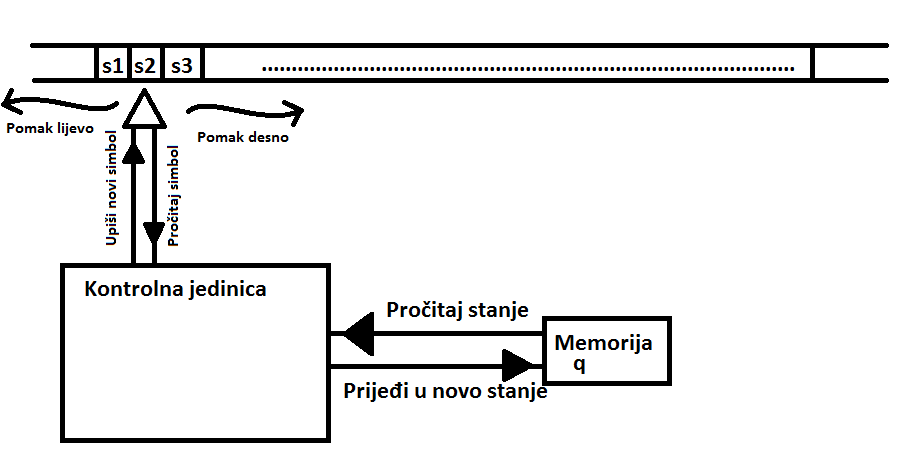
\includegraphics[height=200pt, width=400pt]{Turing.png}
\caption{Shematski prikaz Turingovog stroja}
\label{fig:Turing}
\end{figure} 
\begin{defn}
Neka su $f, g: \N \to \R^{+}$ dvije funkcije. Kažemo da je funkcija $g$ \textbf{asimptotska gornja međa} za funkciju $f$ ako postoje $c>0$ i $n_0 \in \N$ tako da za svaki $n \geq n_0$ vrijedi
\[f(n)\leq cg(n)\]
Činjenicu da je $g$ asimptotska međa od $f$ označavamo sa $f(n)=O(g(n)$. 
\end{defn}
Osnovne definicije (što je alfabet logike sudova, interpretacija, ispunjivost formule, konjunktivna, odnosno, disjunktivna normalna forma  i tako dalje) se mogu naći u \cite[s. ~12-25]{Vukovic}.\\
Više o Turingovom stroju te nekim pojmovima na koje se pozivamo u idućim rezultatima se mogu naći u:
\begin{itemize}
\item Turing prepoznatiljivost, Turing odlučivost \cite[s. ~141-142]{Sipser}
\item Vremenska složenost Turingovog stroja determinističkog se može naći u \cite[s. ~248]{Sipser}, a nedeterminističkog u \cite[s. ~255]{Sipser}
\item Klase vremenske složenosti:
 \begin{itemize}
 	\item $TIME(f(n))$ u \cite[s. ~251]{Sipser}
 	\item $P$  u \cite[s. ~258]{Sipser}
 	\item Vezano uz klasu $NP$ u \cite[s. ~265-267]{Sipser}
 \end{itemize}
 
 	\item Polinomna reducibilnost u \cite[s. ~272]{Sipser}
 	\item NP-potpunost u \cite[s. ~276]{Sipser}
\end{itemize}
Označimo sa $SAT$ skup definiran na idući način:
\[SAT=\{F: F \textrm{ je ispunjiva formula logike sudova }\}\]
Formulacija \textit{problema SAT} glasi:\\
\begin{center}
Za danu formulu logike sudova F koja je u konjunktivnoj normalnoj formi odrediti\\ vrijedi li $F \in  SAT$.
\end{center}
Konjunktivnu normalnu formu koja u svakoj svojoj elementarnoj disjunkciji sadrži točno $k \in \N \backslash \{0\}$ literala nazivamo $k$-knf. Formulacija problema $k-SAT$ glasi:
\begin{center}
	Za proizvoljnu formulu $F$ koja je $k$-knf odrediti je li $F$ ispunjiva. 
\end{center} 
U \cite[s. ~276-283]{Sipser} se može vidjeti da je problem $SAT$ \textit{NP-potpun} problem, kao i $3-SAT$.
Sljedeći teorem govori zapravo o tome da DNA računala, u pogledu vremenske složenosti, imaju bolja svojstva nego deterministički Turnigovi strojevi:
\begin{thm} (Lipton)
Za svaku konjunktivnu normalnu formu $F$ u kojoj se pojavljuje $n$ propozicionalih varijabli i $m$ klauzula, u $\mathcal{O}(m+1)$ separacija i $\mathcal{O}(m)$ spajanja te jednim uočavanjem možemo odlučiti vrijedi li $F \in SAT$
\end{thm}
Dokaz navedenog teorema se može naći u \cite{Lipton}.\\
S pogleda odlučivosti jezika ipak nemamo takav rezultat, odnosno postoji slutnja koja kaže:
\begin{conj} (Kvantna i biološka slutnja) Problem je odlučiv na DNA računalu ili kvantnom računalu ako i samo ako je Turing-odlučiv.
\end{conj}
Postavlja se prirodno pitanje kako izračunati složenost DNA računala. Odgovor je jednostavan: složenost DNA računala procijenjujemo brojem instrukcija koje DNA stroj izvrši, te s kardinalosti skupa $MulS(K)$. Zbog toga što kardinalnost skupa $MulS(K)$ može izrazito brzo rasti (samo jedna operacija \textit{Proširi(K)}, za pripadnu funkciju kratnosti $m$ multiskupa $MulS(K)$ vrijedi da je: $m_{nova}(x):=2\cdot m_{stara}(x)$, gdje je $m_{nova}(x)$ kratnost od $x$ nakon izvršenja operacije \textit{Proširi},a $m_{stara}(x)$ kratnost od $x$ prije izvršenja te iste operacije) prostorna složenost nekog programa za DNA stroj obično doseže nadeksponencijalnu veličinu (vidjet ćemo u idućem podpoglavlju takav slučaj).  
\subsection{Problem Hamiltonovog puta}
\newpage
\nocite{*}
\bibliographystyle{abbrv}
\bibliography{borda2011fundamentals,literatura,CNTYan,lipton}
\end{spacing}
\end{document}